\chapter{SOA}
\label{chap:soa}
Der Begriff SOA ist nicht eindeutig definiert. Je nachdem welche Person man in einem Unternehmen befragt, erhält man unter Umständen eine komplett andere Definition. \frqq Die meisten Definitionen stimmen jedoch zum größten Teil überein und stehen nicht im Konflikt mit einander.\flqq\cite[vgl. Seite 6]{100QA}

Für einen Kaufmann ist SOA etwas Anderes als für einen Analysten. Um die unterschiedlichen Sichten auf SOA besser zu verstehen, werden zunächst einmal einige Definitionen nach \cite{100QA}\ genannt:
\begin{enumerate}
       \item \frqq To the chief information officer (CIO), SOA is a journey that
       promises to reduce the lifetime cost of the application portfolio [...].\flqq \cite[vgl. Seite 6]{100QA}
    
       \item \frqq To the business executive, SOA is a set of services that can be exposed to their customers, partners, and other parts of the organization. Business capabilities, function, and business logic can be combined and recombined to serve the needs of the business now and tomorrow. Applications serve the business because they are composed
       of services that can be quickly modified or redeployed in new
       business contexts, allowing the business to quickly respond to changing
       customer needs, business opportunities, and market conditions.\flqq \cite[vgl. Seite 6]{100QA}
       
       \item \frqq To the business analyst, SOA is a way of unlocking value, because business processes are no longer locked in application silos. Applications no longer operate as inhibitors to changing business needs.\flqq \cite[vgl. Seite 6]{100QA}
       
       \item \frqq To the chief architect or enterprise architect, SOA is a means to
       create dynamic, highly configurable and collaborative applications
       built for change. SOA reduces IT complexity and rigidity. SOA becomes the solution to stop the gradual entropy that makes applications
       brittle and difficult to change. SOA reduces lead times and costs
       because reduced complexity makes modifying and testing applications
       easier when they are structured using services.\flqq \cite[vgl. Seite 6]{100QA}
\end{enumerate}
Jeder der genannten Rollen hat eine eigene Definition von dem was SOA ist. Jede der Definitionen ist jedoch nur ein Teil dessen für was SOA verwendet werden kann, denn SOA ist ein Paradigma und kein festes Modell. Es dient zur Orientierung, gibt jedoch keine feste Richtung vor. Dabei ist das Ziel von SOA nicht die Entwicklung zu vereinfachen oder voran zu bringen, sondern die unternehmensweiten Geschäftsprozesse zu standardisieren und vereinheitlichen.

\section{Business und IT}
\label{sec:BusinessAndIT}
IT darf nie zum Selbstzweck existieren. Sie wird immer zur Unterstützung der Geschäftsprozesse eingesetzt. Oft existieren bereits verschiedene kommerzielle Systeme und Eigenentwicklungen. Mit SOA soll dafür gesorgt werden, dass diese Systeme möglichst effizient miteinander arbeiten können.
\begin{quotation}
    \frqq The complexity of the technology infrastructure at many companies in the financial services sector makes it very hard to leverage IT services in a coordinated way across the enterprise. Many large companies have either merged or acquired other very large companies resulting in the integration of new business units with very different work cultures and widely different information infrastructurse. The need to be able to trust and understand the information about the business across its many disaggregated parts has been a prime motivator for change in the IT infrastructure at these companies.\flqq \cite[S. 17]{SOAForDummies}
\end{quotation}

Mit SOA wird die IT-Infrastruktur eines Unternehmens in zwei Teile geteilt. Auf der einen Seite existiert die Geschäftsschicht mit der Geschäftslogik und auf der anderen Seite die IT-Schicht, welche die Computing-Ressourcen verwaltet. Durch diesen Aufbau ist es nicht nötig, dass ein Business Manager die IT-Schicht verstehen muss.
\\\
In der Geschäftsschicht sind nur Dienste, mit denen Kunden, Lieferanten und Business Partner interagieren. Diese Personen benötigen, genauso wie ein Business Manager, kein Wissen darüber, was in der IT-Schicht existiert oder wie diese aufgebaut ist. Andersherum sind in der IT-Schicht nur Dienste und Applikationen vorhanden, wofür die IT-Abteilung zuständig ist.
\\\\
Damit diese Schichtentrennung funktioniert, wird darauf geachtet, dass in der Geschäftsschicht möglichst wenig Komplexität nach außen sichtbar ist.

\section{Unternehmenskomponenten}
\label{sec:UnternehmensKomponenten}
Unternehmenskomponenten sind ein zentraler Bestandteil von SOA. Die Informationen aus den Komponenten, müssen durch APIs abgerufen werden können. Dienste in einem SOA-System sind nicht, wie anzunehmen, die Unternehmensanwendungen selber, sondern Adapter, welche für die Steuerung der jeweiligen Anwendungen verantwortlich sind. Dabei dient der Adapter nicht nur als API Exposure Gateway, sondern sorgt auch dafür, dass keine Fehlerhaften Anfragen an das System geschickt werden. Spricht man bei SOA von Diensten, ist meistens der Adapter, zusammen mit den Unternehmenskomponenten gemeint. Wird der Begriff "`Dienst"' im Zusammenhang mit SOA verwendet, ist damit der Adapter und die Anwendung bzw. Unternehmenskomponente gemeint.
\\\\
Damit die Geschäftsprozesse mit Hilfe von SOA abgebildet werden können, müssen daher zunächst einmal die dazu gehörenden Komponenten identifiziert werden. beginnend mit den Wichtigsten.

\begin{figure}[htb]
    \centering 
    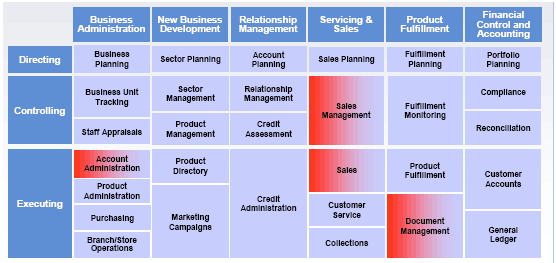
\includegraphics[width=\linewidth]{content/images/UnternehmensKomponenten}\
    \quelle\url{http://www.jot.fm/issues/issue_2008_05/column5/}
    \caption[Unternehmens Komponenten]{Unternehmens Komponenten\\}
    \label{fig:UnternehmensKomponenten}  
\end{figure} 
\newpage
Daraus ergeben sich anschließend die Komponenten, welche untereinander kommunizieren müssen. Die in der Abbildung rot dargestellten Komponenten sind schließlich das Resultat aus der Analyse. Hat man die Komponenten über Kommunikationswege verbunden, werden die nächsten Geschäftsprozesse identifiziert. Diese Prozedur wird solange wiederholt, bis alle Komponenten miteinander verbunden sind.

\section{Enterprise-Service Bus - ESB}
\label{sec:esb}
Der Begriff "`Enterprise-Service Bus"' (ESB) wird oft im Zusammenhang mit SOA verwendet. Der ESB ist jedoch kein Teil von SOA, sondern nur ein Mittel zum Zweck, um die Kommunikation zu vereinheitlichen und ein Exposure Gateway bereitzustellen. Der Enterprise-Service Bus dient dabei als Nachrichtenkomponente, welcher die Nachrichten entgegennimmt und an die jeweiligen Empfänger weiterleitet. Es dient ebenfalls als Transformator von Nachrichten, um die Interoperabilität sicherzustellen. Dabei liegen auf der einen Seite des ESB die Services und auf der anderen Seite die Anwendungen.

\begin{figure}[htb]
    \centering 
    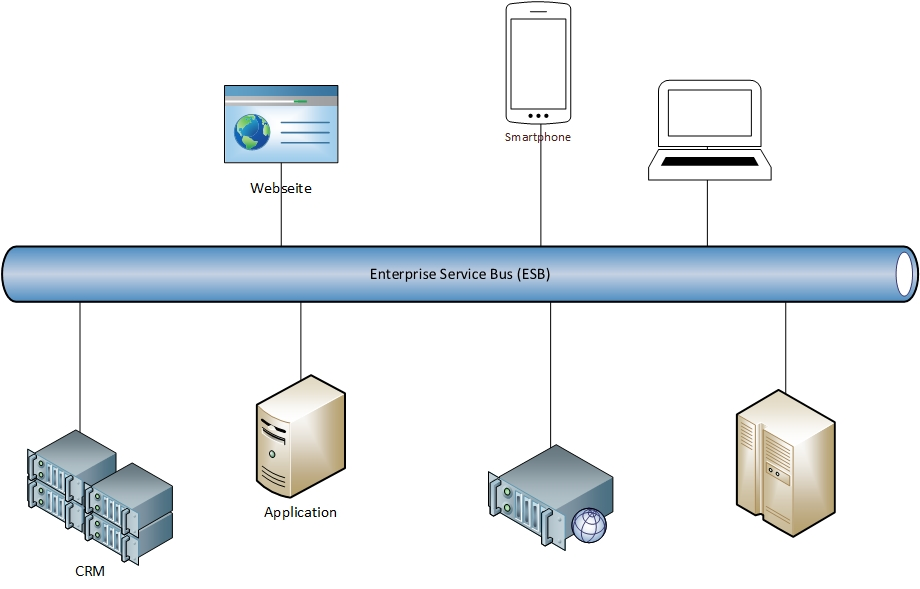
\includegraphics[width=\linewidth]{content/images/ESB}\
    \caption[ESB]{Enterprise Service Bus}
    \label{fig:esb}  
\end{figure}
\newpage
Dienste bieten eine große Menge an Informationen über deren APIs an. Oft werden jedoch nicht alle Informationen benötigt. Gerade auf mobilen Geräten können viele Daten zu langen Ladezeiten führen. Der ESB filtert und bereitet die Daten der Dienste auf und sendet nur die benötigten Daten. Dadurch werden Anwendungen und Anwender nicht mit unwichtigen Daten überfordert.